\documentclass[11pt]{article}
\setlength {\textwidth}{180mm} 
\setlength {\textheight}{260mm}
\topmargin=-35.00mm
\oddsidemargin=-10.00mm
\pagestyle{empty}

\usepackage{graphicx,fancyhdr,natbib,subfigure}
\usepackage{epsfig, epsf}
\usepackage{amsmath, cancel, amssymb}
\usepackage{lscape, longtable, caption}
\usepackage{dcolumn}% Align table columns on decimal point
\usepackage{bm}% bold math
\usepackage{hyperref,ifthen}
\usepackage{verbatim}
\usepackage{color}
\usepackage[usenames,dvipsnames]{xcolor}
%% http://en.wikibooks.org/wiki/LaTeX/Colors



%%%%%%%%%%%%%%%%%%%%%%%%%%%%%%%%%%%%%%%%%%%
%       define Journal abbreviations      %
%%%%%%%%%%%%%%%%%%%%%%%%%%%%%%%%%%%%%%%%%%%
\def\nat{Nat} \def\apjl{ApJ~Lett.} \def\apj{ApJ}
\def\apjs{ApJS} \def\aj{AJ} \def\mnras{MNRAS}
\def\prd{Phys.~Rev.~D} \def\prl{Phys.~Rev.~Lett.}
\def\plb{Phys.~Lett.~B} \def\jhep{JHEP} \def\nar{NewAR}
\def\npbps{NUC.~Phys.~B~Proc.~Suppl.} \def\prep{Phys.~Rep.}
\def\pasp{PASP} \def\aap{Astron.~\&~Astrophys.} \def\araa{ARA\&A}
\def\jcap{\ref@jnl{J. Cosmology Astropart. Phys.}}%
\def\physrep{Phys.~Rep.}

\newcommand{\preep}[1]{{\tt #1} }

%%%%%%%%%%%%%%%%%%%%%%%%%%%%%%%%%%%%%%%%%%%%%%%%%%%%%
%              define symbols                       %
%%%%%%%%%%%%%%%%%%%%%%%%%%%%%%%%%%%%%%%%%%%%%%%%%%%%%
\def \Mpc {~{\rm Mpc} }
\def \Om {\Omega_0}
\def \Omb {\Omega_{\rm b}}
\def \Omcdm {\Omega_{\rm CDM}}
\def \Omlam {\Omega_{\Lambda}}
\def \Omm {\Omega_{\rm m}}
\def \ho {H_0}
\def \qo {q_0}
\def \lo {\lambda_0}
\def \kms {{\rm ~km~s}^{-1}}
\def \kmsmpc {{\rm ~km~s}^{-1}~{\rm Mpc}^{-1}}
\def \hmpc{~\;h^{-1}~{\rm Mpc}} 
\def \hkpc{\;h^{-1}{\rm kpc}} 
\def \hmpcb{h^{-1}{\rm Mpc}}
\def \dif {{\rm d}}
\def \mlim {m_{\rm l}}
\def \bj {b_{\rm J}}
\def \mb {M_{\rm b_{\rm J}}}
\def \mg {M_{\rm g}}
\def \qso {_{\rm QSO}}
\def \lrg {_{\rm LRG}}
\def \gal {_{\rm gal}}
\def \xibar {\bar{\xi}}
\def \xis{\xi(s)}
\def \xisp{\xi(\sigma, \pi)}
\def \Xisig{\Xi(\sigma)}
\def \xir{\xi(r)}
\def \max {_{\rm max}}
\def \gsim { \lower .75ex \hbox{$\sim$} \llap{\raise .27ex \hbox{$>$}} }
\def \lsim { \lower .75ex \hbox{$\sim$} \llap{\raise .27ex \hbox{$<$}} }
\def \deg {^{\circ}}
%\def \sqdeg {\rm deg^{-2}}
\def \deltac {\delta_{\rm c}}
\def \mmin {M_{\rm min}}
\def \mbh  {M_{\rm BH}}
\def \mdh  {M_{\rm DH}}
\def \msun {M_{\odot}}
\def \z {_{\rm z}}
\def \edd {_{\rm Edd}}
\def \lin {_{\rm lin}}
\def \nonlin {_{\rm non-lin}}
\def \wrms {\langle w_{\rm z}^2\rangle^{1/2}}
\def \dc {\delta_{\rm c}}
\def \wp {w_{p}(\sigma)}
\def \PwrSp {\mathcal{P}(k)}
\def \DelSq {$\Delta^{2}(k)$}
\def \WMAP {{\it WMAP \,}}
\def \cobe {{\it COBE }}
\def \COBE {{\it COBE \;}}
\def \HST  {{\it HST \,\,}}
\def \Spitzer  {{\it Spitzer \,}}
\def \ATLAS {VST-AA$\Omega$ {\it ATLAS} }
\def \BEST   {{\tt best} }
\def \TARGET {{\tt target} }
\def \TQSO   {{\tt TARGET\_QSO}}
\def \HIZ    {{\tt TARGET\_HIZ}}
\def \FIRST  {{\tt TARGET\_FIRST}}
\def \zc {z_{\rm c}}
\def \zcz {z_{\rm c,0}}

\newcommand{\ltsim}{\raisebox{-0.6ex}{$\,\stackrel
        {\raisebox{-.2ex}{$\textstyle <$}}{\sim}\,$}}
\newcommand{\gtsim}{\raisebox{-0.6ex}{$\,\stackrel
        {\raisebox{-.2ex}{$\textstyle >$}}{\sim}\,$}}
\newcommand{\simlt}{\raisebox{-0.6ex}{$\,\stackrel
        {\raisebox{-.2ex}{$\textstyle <$}}{\sim}\,$}}
\newcommand{\simgt}{\raisebox{-0.6ex}{$\,\stackrel
        {\raisebox{-.2ex}{$\textstyle >$}}{\sim}\,$}}

\newcommand{\Msun}{M_\odot}
\newcommand{\Lsun}{L_\odot}
\newcommand{\lsun}{L_\odot}
\newcommand{\Mdot}{\dot M}

\newcommand{\sqdeg}{deg$^{-2}$}
\newcommand{\hi}{H\,{\sc i}\ }
\newcommand{\lya}{Ly$\alpha$\ }
%\newcommand{\lya}{Ly\,$\alpha$\ }
\newcommand{\lyaf}{Ly\,$\alpha$\ forest}
%\newcommand{\eg}{e.g.~}
%\newcommand{\etal}{et~al.~}
\newcommand{\lyb}{Ly$\beta$\ }
\newcommand{\cii}{C\,{\sc ii}\ }
\newcommand{\ciii}{C\,{\sc iii}]\ }
\newcommand{\civ}{C\,{\sc iv}\ }
\newcommand{\SiII}{Si\,{\sc ii}\ }
\newcommand{\SiIV}{Si\,{\sc iv}\ }
\newcommand{\mgii}{Mg\,{\sc ii}\ }
\newcommand{\feii}{Fe\,{\sc ii}\ }
\newcommand{\feiii}{Fe\,{\sc iii}\ }
\newcommand{\caii}{Ca\,{\sc ii}\ }
\newcommand{\halpha}{H\,$\alpha$\ }
\newcommand{\hbeta}{H\,$\beta$\ }
\newcommand{\hgamma}{H\,$\gamma$\ }
\newcommand{\hdelta}{H\,$\delta$\ }
\newcommand{\oi}{[O\,{\sc i}]\ }
\newcommand{\oii}{[O\,{\sc ii}]\ }
\newcommand{\oiii}{[O\,{\sc iii}]\ }
\newcommand{\heii}{He\,{\sc ii}\ }
%\newcommand{\heii}{[He\,{\sc ii}]\ }
\newcommand{\nv}{N\,{\sc v}\ }
\newcommand{\nev}{Ne\,{\sc v}\ }
\newcommand{\neiii}{[Ne\,{\sc iii}]\ }
\newcommand{\alii}{Al\,{\sc ii}\ }
\newcommand{\aliii}{Al\,{\sc iii}\ }
\newcommand{\siiii}{Si\,{\sc iii}]\ }


\begin{document}

\title{A Guide to AGN Emission and Absorption Lines and ``What they mean''.}
\author{Nicholas P. Ross}
\date{\today}
\maketitle


\begin{abstract}
This is a (currently very) simple document which will
hopefully/eventually be a pretty complete list of various AGN emission
lines and `what they mean'. That is to say, when a paper reports a
flux of a certain line, why is that line special?
\end{abstract}



\section{Narrow vs. Broad Lines}
{\bf Broad-Line Region.} The lines arising here include hydrogen and helium recombination lines, permitted and semi-forbidden lines such as C IV and [C III (most of these in the emitted UV), and complex multiplets of Fe II. The lack of other lines suggests densities in excess of 10$7$ cm$^{-3}$, and some considerations suggest values as high as 10$^{11}$. At these densities, recombination is a very efficient radiator; a typical BLR requires only 10$^6$ solar masses.

And \href{http://abyss.uoregon.edu/~js/ast123/lectures/lec12.html}{Seyfert Galaxies}. 
The spectra of Seyfert galaxies typically contain:
\begin{itemize} 
  \item{Non-thermal continuum emission;}
  \item{Narrow ($\rightarrow$ low velocity), forbidden ($\rightarrow$ low density material) lines which do not vary detectably ($\rightarrow$ large emitting region)}
      \item{Broad ($\rightarrow$ high velocity), permitted lines which vary on fairly short timescales 
          ($\rightarrow$ small emitting region)}
    \item{ Also, strong emission in the radio, infrared, ultraviolet, and X-ray parts of the spectrum.}
\end{itemize} 

\section{Type 1.5, 1.8 and 1.9s}
%% from https://en.wikipedia.org/wiki/Seyfert_galaxy#Type_1.2.2C_1.5.2C_1.8_and_1.9_Seyfert_galaxies
%Type 1.2, 1.5, 1.8 and 1.9 Seyfert galaxies
%NGC 1275, a type 1.5 Seyfert galaxy

In 1981, Donald Osterbrok introduced the notations Seyfert 1.5, 1.8 and 1.9, where the subclasses are based on the optical appearance of the spectrum, with the numerically larger subclasses having weaker broad-line components relative to the narrow lines. For example, Type 1.9 only shows a broad component in the Hα line, and not in higher order Balmer lines. In Type 1.8, very weak broad lines can be detected in the H$\beta$ lines as well as Hα, even if they are very weak compared to the H$\alpha$. In Type 1.5, the strength of the H$\alpha$ and H$\beta$ lines are comparable.


%% From Roig et al. (2014)
\smallskip
\smallskip
\noindent
From \citet{Roig14}: 
Variations in the relative strength and visibility of the Balmer lines have led some investigators to define more detailed subdivisions of Seyferts. Seyfert 1.5 galaxies have moderate- strength broad H$\alpha$ and H$\beta$; Seyfert 1.8 have weak broad H$\alpha$ and H$\beta$; and Seyfert 1.9 have weak broad H$\alpha$ and only narrow H$\beta$ (see Osterbrock \& Ferland 2006; Ho 2008).



\newpage
\begin{table}
    \caption{Ionization Energies of some (mainly UV) emisson lines}
    \label{tab:Ionization_lines}
    \begin{center}
      \begin{tabular}{lcccr} 
        \hline
        \hline
        Ion            & Wavelength    & Ground  & Ionized  &  Ionization   \\
        name         &  / Angstroms & Level      & Level     &  Energy / eV \\
        \hline
        \hi               & 912                          & $^{2}$S$\frac{1}{2}$       &  n/a                                            &  13.598     \\ 
        \oi               & 1304                        & $^3$P$_2$                     & $2p^3$ $^4$S$^{\circ}_\frac{3}{2}$  &  13.618     \\
        \mgii           & 2800                        & $^{2}$S$_{\frac{1}{2}}$        & $2p^{6}$ $^{1}$S$_{0}$                 &  15.035           \\
        % H$\beta$    & 4861                      &                                 &                                  &            \\ 
        \feii              & 1787                       & $^6$D$\frac{9}{2}$        &    $3d^6$ $^5$D$_4$                  &  16.199          \\
%        \feii              & 1787, 2300-2700   & $^6$D$\frac{9}{2}$        &    $3d^6$ $^5$D$_4$                  &  16.199          \\
        \SiII              &   1260                     & $^2$P$^{\circ}_{\frac{1}{2}}$  &  $3s^2$ $^1$S$_0$                         &  16.345         \\ 
        \alii              & 1671?                          & $^1$S$_0$                        &  $3s$ $^2$S$_{\frac{1}{2}}$  & 	  18.829 \\
        \aliii             & 1857                       & $^2$S$_{\frac{1}{2}}$          & $2p^6$ $^1$S$_{0}$   &    	  28.448 \\  
        \oii               &  3727                      &  $^4$S$^{\circ}_\frac{3}{2}$  &	$2p^2$ $^3$P$_0$ & 35.121                 \\
        % &                &                                 &                                      &            \\ 
%        \hline
        \ciii             & 1909                          & $^1$S$_0$                     & $2s$ $^2$S$_\frac{1}{2}$  &  47.889 \\
        \heii            &  1640                         & $^2$S$_{\frac{1}{2}}$         &   n/a                             & 54.417\\
        \oiii              & 5007                         &  $3$P$0$                     & $ 2p$ $2P°1/2 $          & 54.93554\\
        \civ            & 1548                           &  $^{2}$S$_{\frac{1}{2}}$       & $1s^{2}$ $^{1}$S$_{0}$ &     64.494          \\
        \nv             & 1240                           &  $^{2}$S $_{\frac{1}{2}}$        & $1s^2$ $^1$S$_0$ & 97.890\\
        \hline
                         &                       &             &                &                     \\
                         &                       &             &                &                     \\
        \multicolumn{5}{c}{ From \href{https://ned.ipac.caltech.edu/level5/Sept01/Veilleux/Veilleux5.html}{https://ned.ipac.caltech.edu/level5/Sept01/Veilleux/Veilleux5.html}}\\
        \hline
                         &                       &             &                &                     \\
        Ion            & Wavelength    & Ground  & Ionized  &  Ionization   \\
        name         &  / $\mu$m   & Level      & Level     &  Energy / eV \\
        \hline
        $[\rm{Ca\ VIII}]$    & 2.321 &              &  &	128 \\
	$[\rm{Si\ VI}]$        & 1.962 &              &  &	167 \\
        $\rm{[Si\ VII}]$      & 2.483 &              &  &	205 \\
        $\rm{[Si\ IX}]$      & 3.935 &              &  &	303 \\
	$[\rm{S\ IX}]$          & 1.252             &              &              &	328 \\
        $[\rm{Si\  X}]$    & 1.430            &              &              &	351 \\
        $[\rm{Si\ XI}] $     & 1.932             &              &             &	401 \\
        \hline
        \hline
     \end{tabular}
  \end{center}
\end{table}

\newpage
\begin{table}
  \caption{Ionization Energies of some (mainly UV) emisson lines}
  \label{tab:Ionization_lines}
  \begin{center}
    \begin{tabular}{lcccr} 
      \hline
      \hline
      Ion            & Wavelength    & Ground  & Ionized  &  Ionization   \\
      name         &  / Angstroms & Level      & Level     &  Energy / eV \\
      \hline
      \hi               & 912                          & $^{2}$S$\frac{1}{2}$       &  n/a                            &  13.598     \\ 
      \lyb            &  1025.72                  &  $1s$ $^2$S                   &  $n=3$                               & 12.0875\\
      \lya             & 1215.67                   & $1s$ $^2$S                    &  $n=2$                & 10.198     \\
      \nv             & 1240                           &  $^{2}$S$_{\frac{1}{2}}$        & $1s^2$ $^1$S$_0$ & 97.890\\
      \SiII              &   1260                     & $^2$P$^{\circ}_{\frac{1}{2}}$  &  $3s^2$ $^1$S$_0$                         &  16.345         \\ 
      \oi               & 1304                        & $^3$P$_2$                     & $2p^3$ $^4$S$^{\circ}_\frac{3}{2}$  &  13.618     \\
      \civ            & 1548                           &  $^{2}$S$_{\frac{1}{2}}$       & $1s^{2}$ $^{1}$S$_{0}$ &     64.494          \\
      \heii            &  1640                         & $^2$S$_{\frac{1}{2}}$         &   n/a                             & 54.417\\
      \alii              & 1671?                          & $^1$S$_0$                        &  $3s$ $^2$S$_{\frac{1}{2}}$  & 	  18.829 \\
      \feii              & 1787                       & $^6$D$\frac{9}{2}$        &    $3d^6$ $^5$D$_4$                  &  16.199          \\
      % \feii              & 1787, 2300-2700   & $^6$D$\frac{9}{2}$        &    $3d^6$ $^5$D$_4$                  &  16.199          \\
      \aliii             & 1857                       & $^2$S$_{\frac{1}{2}}$          & $2p^6$ $^1$S$_{0}$   &    	  28.448 \\  
      \ciii             & 1909                          & $^1$S$_0$                     & $2s$ $^2$S$_\frac{1}{2}$  &  47.889 \\
      \mgii           & 2800                        & $^{2}$S$_{\frac{1}{2}}$        & $2p^{6}$ $^{1}$S$_{0}$                 &  15.035           \\
      % H$\beta$    & 4861                      &                                 &                                  &            \\ 
      \oii               &  3727                      &  $^4$S$^{\circ}_\frac{3}{2}$  &	$2p^2$ $^3$P$_0$ & 35.121                 \\
      % &                &                                 &                                      &            \\ 
      % \hline
      \oiii              & 5007                         &  $3$P$0$                     & $ 2p$ $2P°1/2 $          & 54.93554\\
      \hline
        \hline
     \end{tabular}
  \end{center}
\end{table}


\newpage
\begin{figure}
  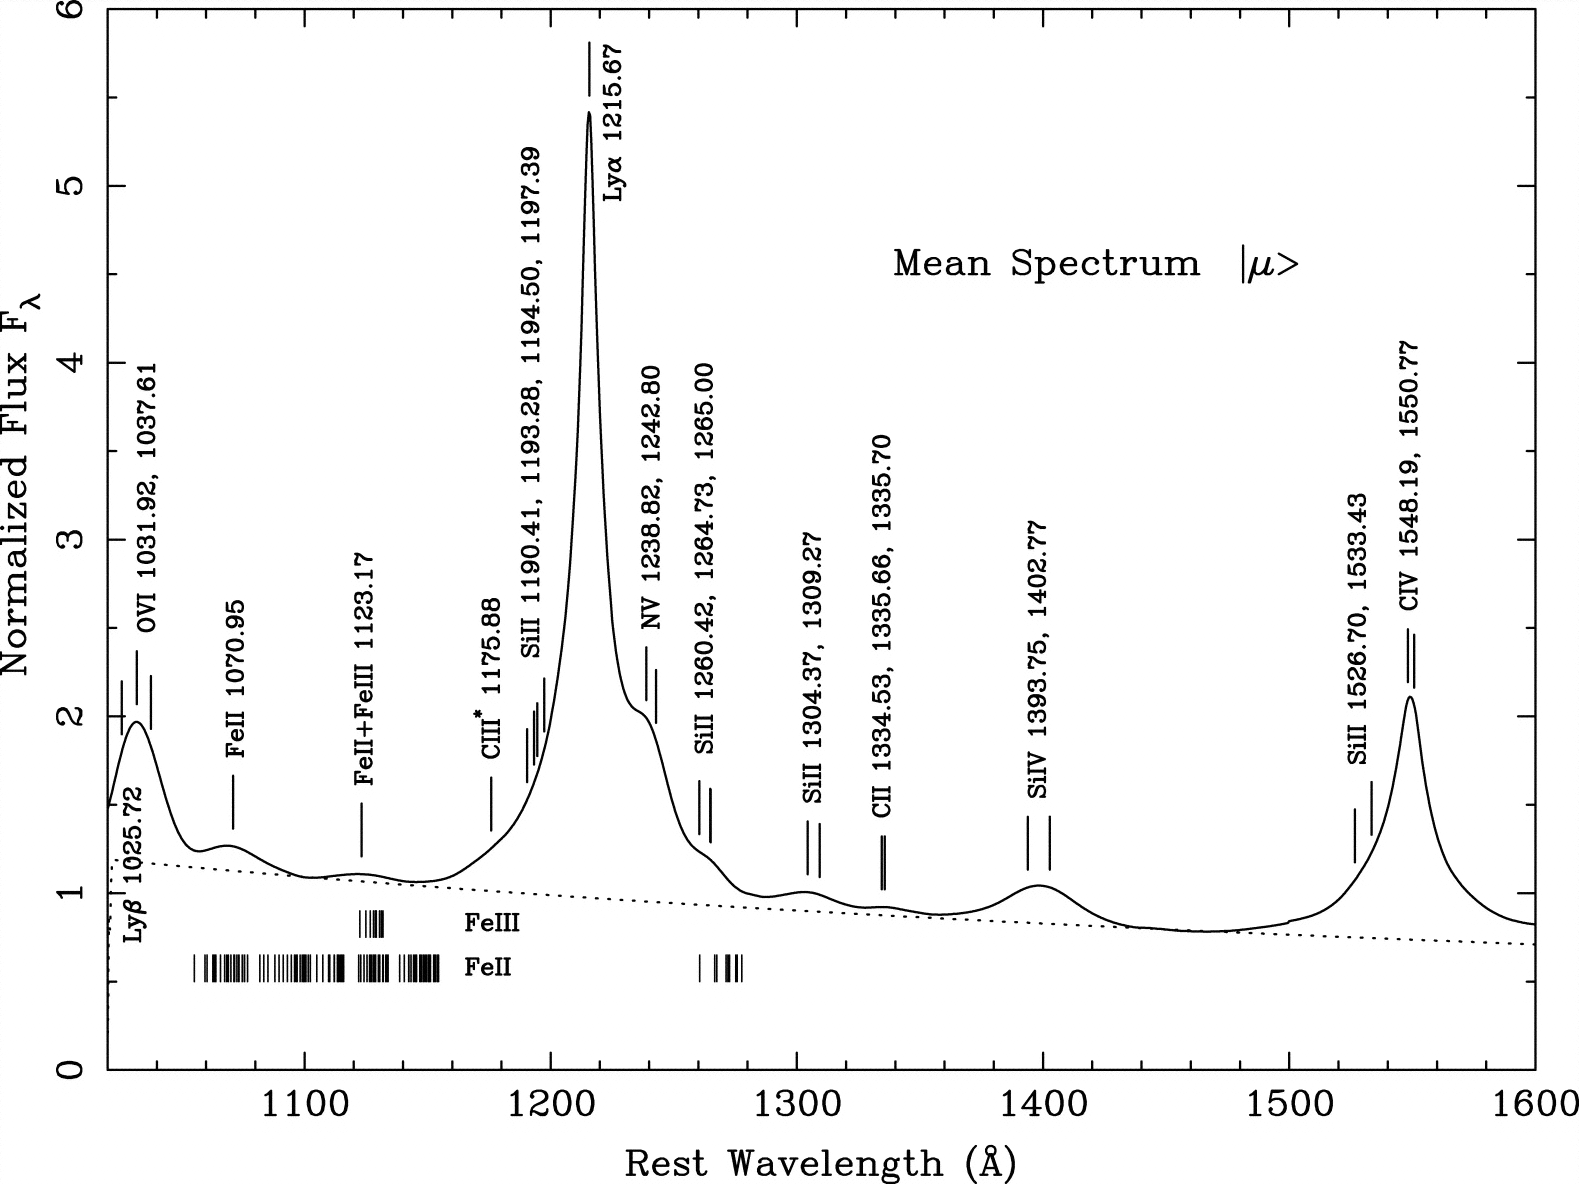
\includegraphics[height=10.0cm,width=12.0cm, angle=270]{Suzuki_2005_Fig1.png}
  \centering
  \caption[]{
From \citet{Suzuki05}: Mean spectrum of 50 HST quasar spectra. The
spectrum is normalized near 1280\AA. The wavelengths are taken from
Morton (1991), except for \feii, \feiii, and \ciii$^*$ lines, which
are observed wavelengths from Tytler et al. (2004a). The tick marks
shown below the spectrum are the wavelengths of the \feii and \feiii
multiplet. The dotted line is the power-law continuum
approximation. Note that the emission lines do exist in the \lya
wavelength region. We also note that the wavelength separation of the
\SiIV doublet at $\lambda$1400 is relatively large and makes the line
profile broad.
}
  \label{fig:fig1}
\end{figure}


\section{Ionization Line}
NIST is your friend!!!\\
\href{http://physics.nist.gov/PhysRefData/ASD/ionEnergy.html}{http://physics.nist.gov/PhysRefData/ASD/ionEnergy.html}\\

%%  E (eV) = 1239.84193 eV nm / lambda (nm)
%%  energy_in_eV = 1239.84193/(1./(inv_cms*1e-7))

\noindent
THIS LINK!!!:\\
\href{https://dept.astro.lsa.umich.edu/~cowley/ionen.htm}{https://dept.astro.lsa.umich.edu/~cowley/ionen.htm}\\

\noindent
And also, \\
\href{http://www.pa.uky.edu/$\sim$verner/atom.html}{http://www.pa.uky.edu/$\sim$verner/atom.html}\\


     \subsection{High-Ionization Line}
     From Wu et al. (2012)
    ``...are clearly AGNs as evidenced by strong, high-ionization emission lines such as O vi, C iv, and/or C iii].''\\

    ``High-ionization BALQSOs ( HiBALs) contain strong, broad absorption troughs shortward of high-ionization emission lines and are typically identified through the presence of \civ absorption troughs \citep{Trump06}.''
    

     \subsection{Low-Ionization Line}
     ``LoBALs are QSOs that have BALs from ions at lower ionization states such as \aliii or \mgii''  \citep{Gibson09}


\begin{landscape}
\begin{table}
  \caption{The Lines}
  \label{tab:the_lines}
  \begin{center}
    \begin{tabular}{lrllll} 
      \hline
      \hline
      Name & Wavelength / \AA & Transition & Rest Passband & 
      Interpreation & Reference \\
      \hline
      Lyman-$\alpha$ & 1215.67 & 2 to 1        & $\sim$FUV & Major QSO line       & 1 \\
      Lyman-$\beta$  & 1025.18 & 3 to 1        & $\sim$FUV &        & 1 \\
      Lyman-$\gamma$ &  972.02 & 4 to 1        & $\sim$FUV &        & 1 \\
      Lyman Limit    &  911.27 & $\infty$ to 1 & $\sim$FUV &        & 1 \\
      \hline
      H-$\alpha$     & 6563.   & 3 to 2        & R,r       & Recent major SF or AGN activity & 2 \\
      H-$\beta$      & 4861.   & 4 to 2        & B,V,g     &  & 2 \\
      H-$\gamma$     & 4341.   & 5 to 2        & U,B,u     &  & 2 \\
      H-$\delta$     & 4102.   & 6 to 2        & $\sim$FUV & Previous SF history  & 3 \\
      Balmer Limit   & 3646.   & $\infty$ to 2 & $\sim$FUV &  & 2 \\
      \hline
      HI              & 3646.   & $\infty$ to 2 & $\sim$FUV &  & 2 \\
      HII             & 3646.   & $\infty$ to 2 & $\sim$FUV &  & 2 \\
      \hline
      HeI              & 3646.   & $\infty$ to 2 & $\sim$FUV &  & 2 \\
      HeII             & 3646.   & $\infty$ to 2 & $\sim$FUV &  & 2 \\
      HeIII            & 3646.   & $\infty$ to 2 & $\sim$FUV &  & 2 \\
      \hline
      CIV              & 3646.   & $\infty$ to 2 & $\sim$FUV & Major QSO line & 2 \\
      \hline
      OII              & 3646.   & $\infty$ to 2 & $\sim$FUV & Major QSO line & 2 \\
      \hline
      OIII             & 3646.   & $\infty$ to 2 & $\sim$FUV & Recent major SF line & 2 \\ 
      OIII             & 5007.   & $\infty$ to 2 & $\sim$FUV & Recent major SF line & 2 \\
      \hline
      Ca II H          & 3999.   & $\infty$ to 2 & $\sim$FUV & Old stellar pop & 3 \\
      Ca II K          & 4001.   & $\infty$ to 2 & $\sim$FUV & Old stellar pop & 3 \\
      \hline
      NII              & 5007.   & $\infty$ to 2 & $\sim$FUV &  & 2 \\
      \hline
      NeV              & 3646.   & $\infty$ to 2 & $\sim$FUV & Major QSO line & 2 \\
      \hline
      $[$OIII $\lambda$ 5007/ H$\beta]$ &   &  &   & ``BPT'' diagram reliable tool for determining source & 2, 4, 5 \\
      $[$NII $\lambda$ 6583/ H$\alpha]$ & & & & of line emission from a galaxy visually differentiate & 2,4,5 \\
                                      & & & & between Seyferts, LINERs and SF gals. However, only at & \\
                                      & & & & ``low'' redshifts since need H$\alpha$, (not at $z\sim1$). & \\
                                      & & & &  Modified BPT with $(U-B)$ colour replacing & \\
                                      & & & & $[$NII $\lambda$ 6583/ H$\alpha]$ e.g. Montero-Dorta, 0801.2769. & \\
      \hline
      [SII $\lambda$ 6583/ H$\alpha$]   &    & $\infty$ to 2 & $\sim$FUV & Major QSO line & 2,4. 5  \\
      \hline
      [$\alpha$/Fe]             & 3646.   & $\infty$ to 2 & $\sim$FUV & Major QSO line & 2 \\
      \hline
      NV               & 1???.67 & 2 to 1        & $\sim$FUV & Major QSO line       & 1 \\
      SiIV             & 1???.67 & 2 to 1        & $\sim$FUV & Major QSO line       & 1 \\
      CIV              & 1???.67 & 2 to 1        & $\sim$FUV & Major QSO line       & 1 \\
      CIII]            & 1???.67 & 2 to 1        & $\sim$FUV & Major QSO line       & 1 \\
      MgII             & 1???.67 & 2 to 1        & $\sim$FUV & Major QSO line       & 1 \\
      \hline
      \hline
% GALEX FUV: 1350-1750, % GALEX NUV: 1750-2800
%Lyman alpha forest is the sum of absorption lines arising from the Lyman alpha transition of the neutral hydrogen in the spectra of distant galaxies and quasars.
    \end{tabular}
  \end{center}
\end{table}
\end{landscape}


\newpage
\section{CLAGN and CLQ Mini-lit review} 
This is just a quick section for a mini CLAGN and CLQ literature review. 
A lot of these references are from Steph LaMassa's ``Hidden Monsters'' talk:
\href{http://www.dartmouth.edu/~hiddenmonsters/presentations\_tab.php}{http://www.dartmouth.edu/~hiddenmonsters/presentations\_tab.php}\\

\noindent
\citet{TohlineOsterbrock76} for NGC 7603.\\
\citet{PenstonPerez84} for NGC 4151.\\
\citet{Goodrich95} for NGC 4151.\\
\citet{Tran92}\\
\citet{Storchi-Bergmann93}\\
\citet{EracleousHalpern01}\\
\citet{Shappee14}\\
\citet{Aretxaga99} for NGC 7582.\\
\citet{Denney14} for Mrk 590.\\



\newpage
\section{MgII} 
This is just a quick mini-section on the MgII line. 




\begin{table}
  \caption{The Lines, in increasing Wavelength (Basis for this table from 
  SDSS SkyServer Schema Browser, SpecLineNames view {\tt http://casjobs.sdss.org/dr6/en/help/browser/browser.asp}) }
  \label{tab:the_lines}
  \begin{center}
    \begin{tabular}{lll} 
      \hline
      \hline
name &	value &	description \\
      \hline
UNKNOWN	   &    0    & 	0.00 \\
OVI\_1033   &	1033 &	1033.82 \\
Lya\_1215   &	1215 &	1215.67 \\
NV\_1241    &   1241 &	1240.81 \\
OI\_1306    &   1306 &	1305.53 \\
CII\_1335   &	1335 &	1335.31 \\
SiIV\_1398  &	1398 &	1397.61 \\
SiIV\_OIV\_1400 & 1400 &  1399.80 \\
CIV\_1549   &   1549 &	1549.48 \\
HeII\_1640  &	1640 &	1640.40 \\
OIII\_1666  &	1666 &	1665.85 \\
AlIII\_1857 &	1857 &	1857.40 \\
CIII\_1909  &	1909 &	1908.73 \\
CII\_2326   &	2326 &	2326.00 \\
NeIV\_2439  &	2439 &	2439.50 \\
MgII\_2799  &	2799 &	2799.12 \\
NeV\_3347   &	3347 &	3346.79 \\
NeV\_3427   &	3427 &	3426.85 \\
OII\_3727   &	3727 &  3727.09 \\
OII\_3730   &	3730 &	3729.88 \\
Hh\_3799    &   3799 &  3798.98 \\
Oy\_3836    &   3836 &	3836.47 \\
HeI\_3889   &	3889 &	3889.00 \\
CaII K\_3935 &  3935 &	3934.78 \\
CAII H\_3970 &  3970 &	3969.59 \\
He\_3971    &   3971 &	3971.19 \\
SII\_4072   &	4072 &	4072.30 \\
Hd\_4103    &   4103 &	4102.89 \\
G\_4306	    &   4306 &	4305.61 \\
Hg\_4342    &   4342 &	4341.68 \\
OIII\_4364  &	4364 &	4364.44 \\
Hb\_4863    &   4863 &  4862.68 \\
OIII\_4933  &	4933 &	4932.60 \\
OIII\_4960  &	4960 &  4960.30 \\
OIII\_5008  &	5008 &  5008.24 \\
Mg\_5177    &   5177 &	5176.70 \\
Na\_5896    &   5896 &	5895.60 \\
OI\_6302    &   6302 &	6302.05 \\
OI\_6366    &   6366 &	6365.54 \\
NI\_6529    &   6529 &	6529.03 \\
NII\_6550   &	6550 &	6549.86 \\
Ha\_6565    &   6565 &	6564.61 \\
NII\_6585   &	6585 &	6585.27 \\
Li\_6708    &   6708 &	6707.89 \\
SII\_6718   &	6718 &	6718.29 \\
SII\_6733   &	6733 &	6732.67 \\
CaII\_8500  &   8500 &	8500.36 \\
CaII\_8544  &	8544 &	8544.44 \\
CaII\_8665  &	8665 &	8664.52 \\
      \hline
      \hline
 \end{tabular}
   \end{center}
\end{table}


\section{Notes, Links and To Dos...}


\section{``Manual'' References and Links}
Morton, D. C. 1991, ApJS, 77, 119
Tytler, D., O’Meara, J. M., Suzuki, N., Kirkman, D., Lubin, D., \& Orin, A.. 2004a, AJ, 128, 1058

see also:: \\ 
https://arxiv.org/abs/1703.04250v1

\bibliographystyle{mn2e}
\bibliography{/cos_pc19a_npr/LaTeX/tester_mnras}

\end{document}

